\subsection{SMP}
Pour encore gagner de la puissance, nous pouvons connecter plusieurs processeurs ensemble.
%
Ces processeurs se partagent les ressources disponibles sur la carte mère, cela inclut les entrées/sorties et la mémoire.
%
La façon d'inter-connecter tous les processeurs avec la carte mère peut différer entre différentes architectures.
%
Avec l'architecture SMP, tous les processeurs sont connectés à un bus de données et un arbitre choisit quel processeur peut utiliser le bus à un instant donné (Fig.~\ref{fig:smp}).
%
Cette conception ne passe pas à l'échelle au niveau des performances quand le nombre de processeurs grandit.
%
La bande passante est partagée par tous les processeurs et l'arbitre du bus devient un goulot d'étranglement.
%
Pire, la latence d'un accès mémoire va dépendre de la congestion du bus mémoire.
%
L'utilisation de 4 processeurs comme décrit précédemment donne une puissance de calcul de 256~GLOPS.
%
Cette puissance de calcul ne prend pas en compte les limitations mémoires.
%
Pour pouvoir atteindre cette puissance, il faut limiter les accès à la mémoire partagée et privilégier les accès à la mémoire cache.


%   (-_-)   %
\begin{figure}[!ht]
        \centering
        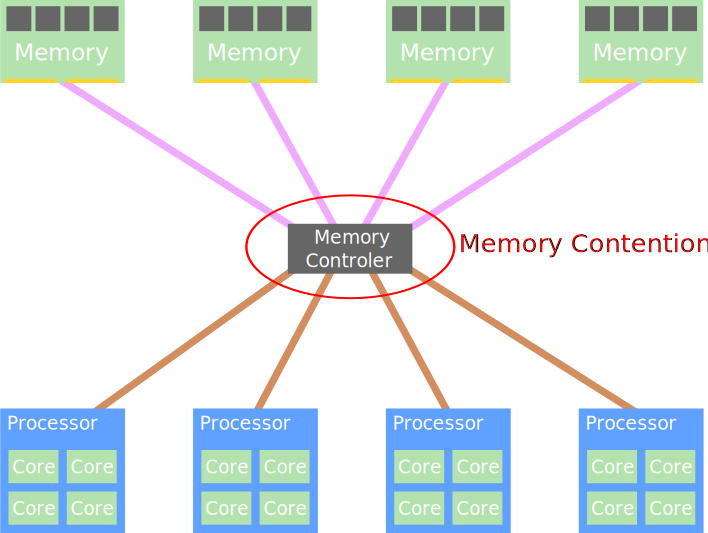
\includegraphics[width=0.8\textwidth]{smp}
        \caption{Vue d'ensemble d'une architecture à accès mémoire uniforme (SMP).}
        \label{fig:smp}
\end{figure}
